\documentclass[twoside]{article}

\usepackage{mystyle}
\usepackage{tikz}
\usetikzlibrary{positioning}

\usepackage[group-separator={,},group-minimum-digits={4}]{siunitx}

\title{Machine Learning for Data Science - Competition 2}
\author{Antoine Klopocki, Jaydev Kshirsagar, Travis Westura, Vishisht Tiwari\\Kaggle Team Name: Antravishjay}
\date{\vspace{-5ex}} % vspace hack to remove date without looking into titling package

\begin{document}

\maketitle
\thispagestyle{empty}

\section{Introduction}\label{sec:introduction}

In this competition we are given a robot that is moving around in~$\R^2$.
The robot makes $\num{10000}$~runs, and for $\num{1000}$~timesteps we observe the angle~$\theta$ that the robot's position makes with the $x$-axis.
But are not given the robot's precise ${(x, y)}$~location, and the angle itself does not determine directly the robot's position.
The true position could be anywhere along the line passing through the origin and making angle~$\theta$ with the $x$-axis.

Our task is to determine the robot's ${(x, y)}$-position on the $\num{1001}$st~timestep as accurately as possible, with accuracy determined by Root Mean Square Error.
Our methods achieve an accuracy score of~$\bm{0.26233}$.

\section{Determining the Observer's Position}\label{sec:determ-observ-posit}

The competition specification describes the robot moving in the first quadrant, and the angles given in the observations file contain the angle made between the robot's location~${(x_{r, t}, y_{r, t})}$ and the $x$-axis.
However, the coordinates given in the label file contain coordinates with negative values.
We'll denote to these values as~${(x_{r, t}', y_{r, t}')}$.
Since these values are negative, the observer of the locations is positioned in the first quadrant as well, and we call it's location~${(a, b)}$.
First we need to determine the coordinates of this point so that we can match up the data in the observation and label files.

Consider a labeled point~${(x_{r, t}', y_{r, t}')}$.
The angle~$\theta$ that this point forms with the $x$-axis is given by
\begin{equation*}
  \tan\theta = \frac{b + y_{r, t}'}{a + x_{r, t}'}.
\end{equation*}
We know the value of $\theta$ from the observations file.
Since there are two unknowns $a$~and~$b$, we pick two labeled points and solve the system of equations
\begin{equation*}
  \tan\theta_1 = \frac{b + y_{r_1, t_1}'}{a + x_{r_1, t_1}'}, \quad \tan\theta_2 = \frac{b + y_{r_2, t_2}'}{a + x_{r_2, t_2}'}.
\end{equation*}
We use the points from run~$1$ time steps $205$~and~$216$.
Solving the system of equations yields the position of the location observer as~$(1.5, 1.5)$.
Using this position, we consider the observation angles as being measured at~$(0, 0)$.

Further, we can use the $\num{600000}$ labeled points to gain intuition about the robot's movement.
We compute the average of radius of these points to $(1.5, 1.5)$ to see that this average is approximately~$1$.
Plotting the labeled points in \cref{fig:label-locations}, we see that the robot is moving roughly in a circle of radius~$1$ centered at~$(1.5, 1.5)$, with kinks occurring at the top, bottom, left, and right of the circle.
\begin{figure}[h]
  \centering
  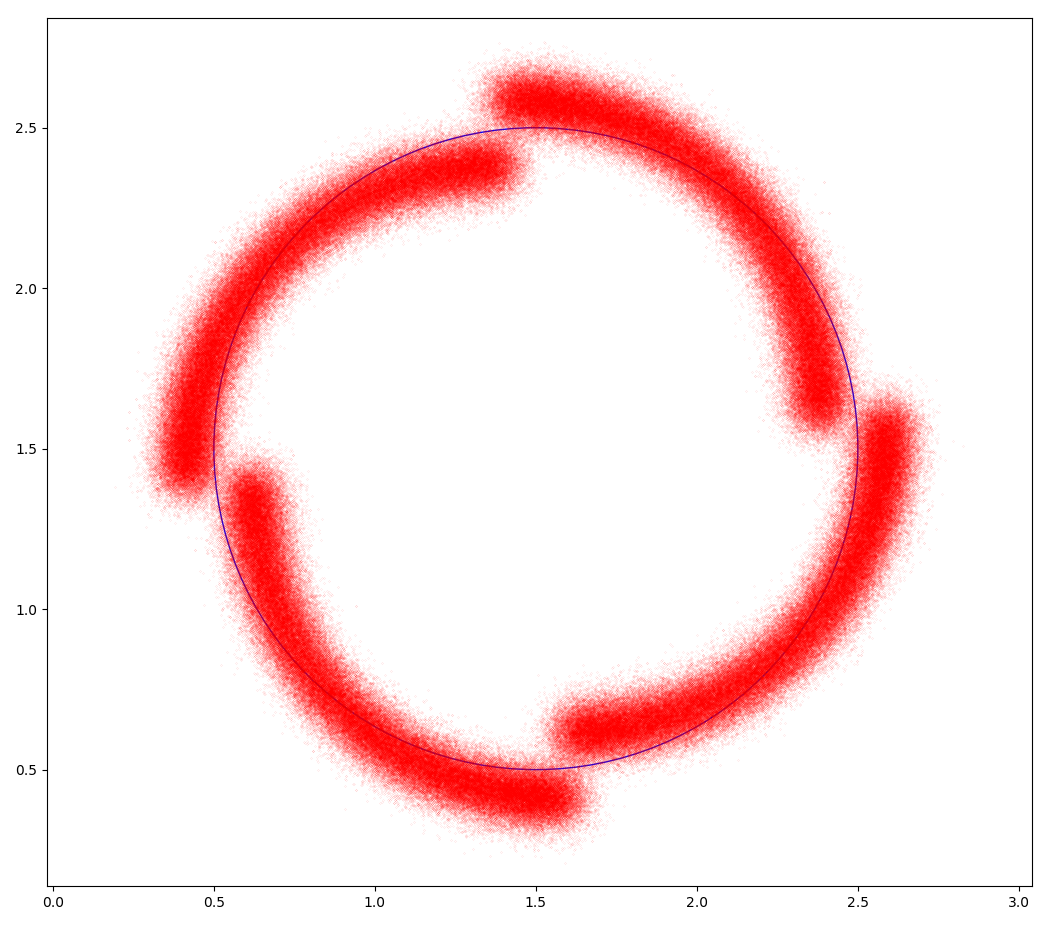
\includegraphics[width=0.5\textwidth]{images/label-locations}
  \caption{Locations of the robot given as labels.}\label{fig:label-locations}
\end{figure}

Every run starts the robot at~$(1.5, 1.5)$.
But we are not given any labels for the first $200$~runs, and we see that the robot stabilizes into its standard path by the time we start obtaining labels for its location.

\section{Hidden Markov Models (HMM's)}\label{sec:hidden-markov-models}

We represent this problem as a Hidden Markov Model.
A Hidden Markov Model is a graphical model with two types of variables: latent variables~$S_t$ and observed variables~$X_t$.
The latent variables represent states that are not visible to the observer.
Each observed variable~$X_t$ depends only on the corresponding state variable~$S_t$.
And each state variable~$S_t$ depends only on the previous state variable~$S_{t-1}$.
We depict latent variables as shaded vertices.

\begin{figure}[h]
  \centering
  \tikz[]{
    \node[draw, circle, fill=gray] (S1) {$S_1$};
    \node[draw, circle] (X1) [on grid, below = 1.5cm of S1] {$X_1$};
    \node[draw, circle, fill=gray] (S2) [on grid, right = 1.5cm of S1] {$S_2$};
    \node[draw, circle] (X2) [on grid, below = 1.5cm of S2] {$X_2$};
    \node[] (dots) [right = 0.7cm of S2] {$\cdots$};
    \node[draw, circle, fill=gray] (Sn) [on grid, right = 1.5cm of dots] {$S_T$};
    \node[draw, circle] (Xn) [on grid, below = 1.5cm of Sn] {$X_T$};

    \path[shorten >=0.1cm, shorten <=0.1cm, ->] (S1) edge (X1);
    \path[shorten >=0.1cm, shorten <=0.1cm, ->] (S1) edge (S2);
    \path[shorten >=0.1cm, shorten <=0.1cm, ->] (S2) edge (X2);
    \path[shorten >=0.1cm, shorten <=0.1cm, ->] (S2) edge (dots);
    \path[shorten >=0.1cm, shorten <=0.1cm, ->] (dots) edge (Sn);
    \path[shorten >=0.1cm, shorten <=0.1cm, ->] (Sn) edge (Xn);
  }
  \caption{Hidden Markov Model}\label{fig:hmm}
\end{figure}

In our problem the observed values are the angles that the robot's position makes with the $x$-axis.
The robot is moving around in the plane~$\R^2$.
This space is continuous, so our observations are angles in the continuous range~$\big(0, \frac{\pi}{2}\big)$.
We discretize this space in order to use a Hidden Markov Model.
We divide the first quadrant into $K$~sectors, ${\textstyle \big[0, \frac{1}{K}\frac{\pi}{2}\big), \big[\frac{1}{K}\frac{\pi}{2}, \frac{2}{K}\frac{\pi}{2}\big), \ldots, \big[\frac{K - 1}{K}\frac{\pi}{2}, \frac{\pi}{2}\big)}$, where $K$ is a parameter that we choose.
The observation, rather than being a value in $\big(0, \frac{\pi}{2}\big)$, is instead given by an integer~${1, 2, \ldots, K}$ representing the segment of the interval in which the angle lies.
As a further refinement of this technique, we find the minimum and maximum angles that occur in the observations file, $\theta_{\text{min}}$~and~$\theta_{\text{max}}$, and divide the shorter interval~$[\theta_{\text{min}}, \theta_{\text{max}}]$.
\begin{wrapfigure}{o}{0.5\textwidth}
  \begin{center}
    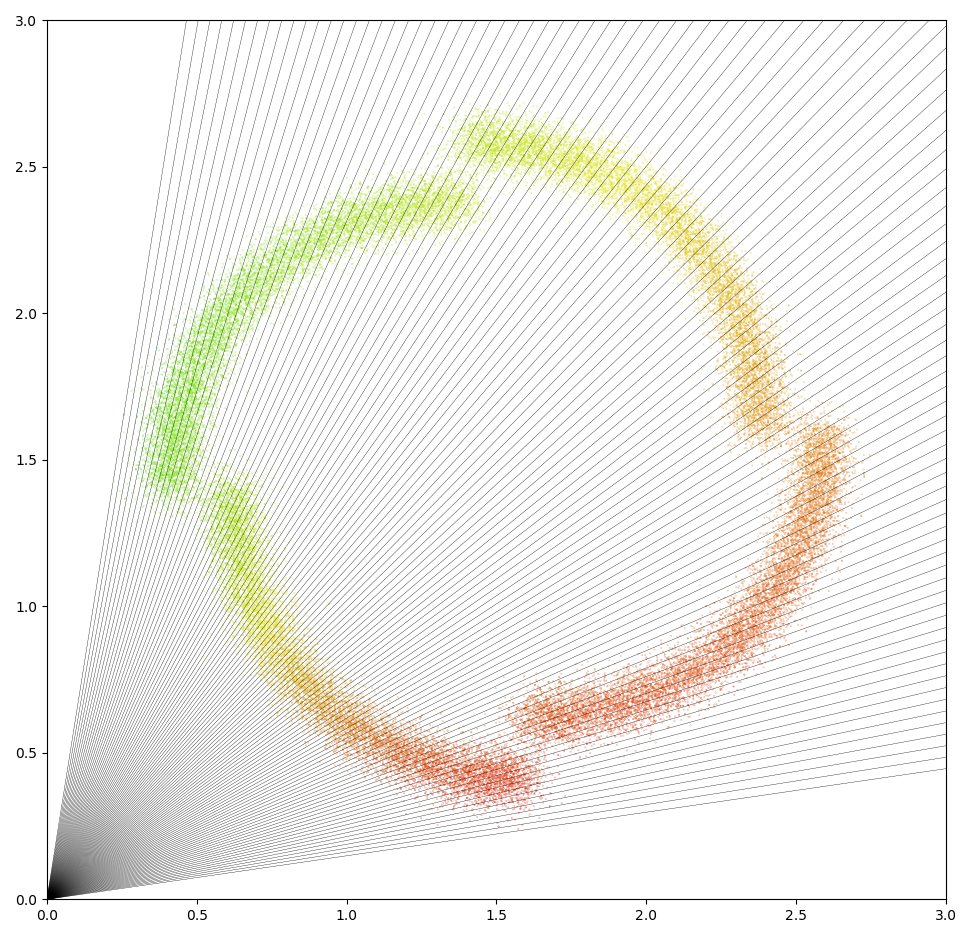
\includegraphics[width=0.48\textwidth]{images/angle-discrete}
    \caption{Labeled points colored based on the segment in which they lie with~${K = 100}$.}
  \end{center}
\end{wrapfigure}

Given an observation and the corresponding state, we need to map the state to the robot's position.
We outline a procedure for doing this in . % TODO give section number when the section is written

Given the observations, we need to estimate the transition matrix~$A$ and emission matrix~$B$ of the Hidden Markov Model.
The transition matrix is defined by
\begin{equation*}
  a_{i,j} = \Pr(S_{t} = j \mid S_{t-1} = i),
\end{equation*}
that is, each entry~$a_{i, j}$ gives the probability of being in state~$i$ given that the previous state is state~$j$.
With $N$~states, $A$ is an ${N \times N}$-matrix.
The emission matrix is defined by
\begin{equation*}
  b_{i, k} = \Pr(X_t = k \mid S_t = i),
\end{equation*}
that is, each entry~$b_{i, k}$ gives the probability of the observation~$k$ being emitted given state~$i$.
With $N$~states and $K$~possible observations, $B$ is an ${N \times K}$-matrix.
In~\cref{sec:baum-welch} we describe our process for estimating these matrices using the Baum Welch algorithm.

\section{Baum Welch}\label{sec:baum-welch}

The Baum Welch algorithm is an Expectation Maximization (EM) algorithm for learning the parameters of Hidden Markov Models.
We use a forward-backwards algorithm to perform inference for the expectation step and then update the HMM parameters in the maximization step.
We thereby find the maximum likelihood estimate of the parameters of the model.
The algorithm takes as parameters a triple~$(A, B, \pi)$, where $A$~and~$B$ are the transition and emission matrices and $\pi$ is the initial state distribution, that is, the probability of the first state being state~$i$ is given by ${\pi_i = \Pr(S_1 = i)}$.

\subsection{Explanation of Algorithm}\label{sec:expl-algor}

Let $N$ be the number of states, $K$ be the number of observations, and $T$ be the number of time steps.

For the forward procedure we calculate ${\alpha_i(t) = \Pr(X_1 = x_1, X_2 = x_2, \ldots, X_t = x_t, S_t = i \mid A, B, \pi)}$, which is the probability of obtaining observations~${y_1, y_2, \ldots, y_t}$ and being in state~$i$ at time~$t$.
We recursively compute
\begin{align*}
  \alpha_i (t) &:= \pi_i b_{i, x_1},\\
  \alpha_i (t + 1) &:= b_{i, x_{t+1}} \sum_{j=1}^N \alpha_j(t) a_{j, i}.
\end{align*}
For the backward procedure we calculate ${\beta_i(t) = \Pr(X_{t+1} = x_{t+1}, \ldots, X_T = x_T \mid S_t = i, A, B, \pi)}$, the probability of the observations ${x_{t+1}, \ldots, x_T}$ occurring given the $t$th~state is state~$i$.
Again we compute recursively to set
\begin{align*}
  \beta_i(T) &:= 1,\\
  \beta_t(t) &:= \sum_{j=1}^N \beta_j(t+1) a_{i, j} b_{j, x_{t+1}}.
\end{align*}

Before performing the updates, we first calculate two temporary variables.
We define $\gamma_i(t)$ to be the probability of being in state~$i$ at time~$t$ given a set of observations~${X = (X_1 = x_2, \ldots, X_T = x_T)}$.
Applying Bayes's theorem we have
\begin{equation*}
  \gamma_i(t) := \Pr(S_t = i \mid X, A, B, \pi) = \frac{\Pr(S_t = i, X \mid A, B, \pi)}{\Pr(X \mid A, B, \pi)} = \frac{\alpha_{i}(t) \beta_i(t)}{\sum_{j = 1}^N \alpha_j(t) \beta_j(t)}.
\end{equation*}
Next we define $\xi_{i, j}(t)$ to be the probability of being in state~$i$ at time~$t$ and state~$j$ at time~$t + 1$ given a sequence of observations~$X$ with parameters $A$,~$B$, and~$\pi$.
\begin{align*}
  \xi_{i, j}(t) &:= \Pr(S_t = i, S_{t+1} = j \mid X, A, B, \pi) = \frac{\Pr(S_t = i, S_{t+1} = j, X \mid A, B, \pi)}{\Pr(X \mid A, B, \pi)},\\
  &= \frac{\alpha_t(t) a_{i, j} \beta_j(t + 1) b_{j, t+1}}{\sum_{i=1}^N \sum_{j=1}^N \alpha_i(t) a_{i, j} \beta_j(t+1) b_{j, t+1}}.
\end{align*}
We use these temporary variables to update the parameters of our Hidden Markov Model.
The vector~$\pi$ is updated so each entry~$\pi_i$ is the probability of being in state~$i$ at the first time~${t = 1}$.
\begin{equation*}
  \pi_i := \gamma_i(1)
\end{equation*}
The values~$a_{i, j}$ are updated to be the expected number of transitions from state $i$~to~$j$ divided the total number of transitions from~$i$ (including from $i$ back to itself).
\begin{equation*}
  a_{i, j} := \frac{\sum_{t=1}^{T-1}\xi_{i, j}(t)}{\sum_{t=1}^{T-1}\gamma_i(t)}
\end{equation*}
And finally the values~$b_{i, k}$ is set to the expected number of times the observation~$k$ is emitted from state~$i$ over the total number of times state~$i$ occurs.
\begin{equation*}
  b_{i,k} := \frac{\sum_{t=1}^T \1_{X_t = k}\gamma_i(t)}{\sum_{t=1}^T \gamma_i(t)}
\end{equation*}

\subsection{Numerical and Running Time Issues}\label{sec:numer-runn-time}

\subsection{Choice of Parameters}\label{sec:choice-parameters}

\begin{figure}[h]
  \centering
  \begin{subfigure}[h]{0.48\textwidth}
    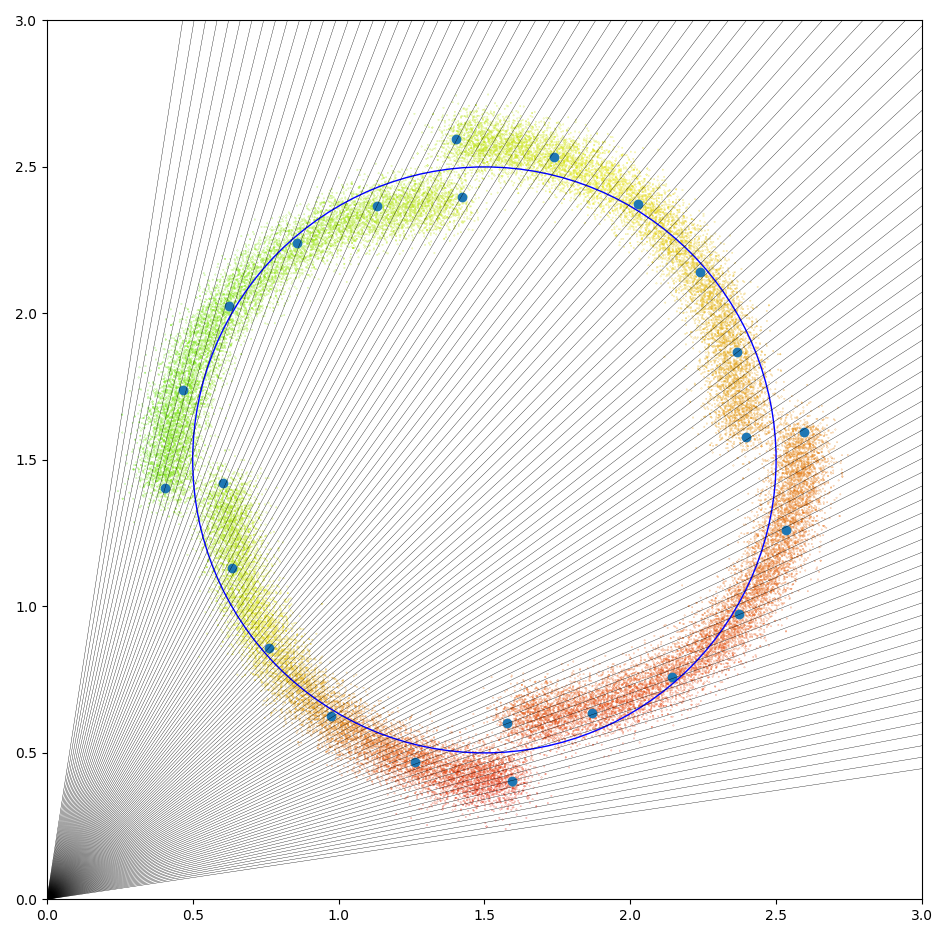
\includegraphics[width=\textwidth]{images/init-states-24}
    \caption{N = 24.}\label{fig:24-states}
  \end{subfigure}
  \begin{subfigure}[h]{0.48\textwidth}
    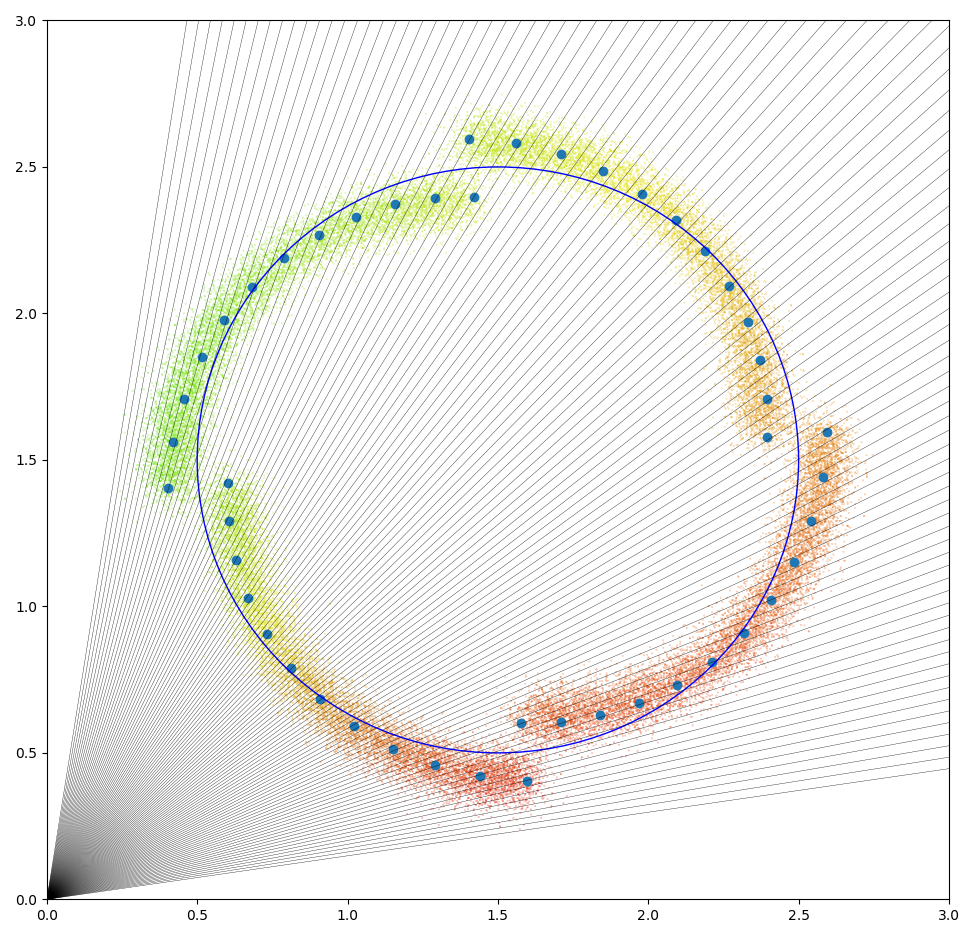
\includegraphics[width=\textwidth]{images/init-states-48}
    \caption{N = 48.}\label{fig:48-states}
  \end{subfigure}
  \caption{Initial state positions for different numbers of states.}\label{fig:init-trans-pos}
\end{figure}

\section{Viterbi}\label{sec:viterbi}



\end{document}

